
\chapter{Design and Implementation of Air pollution Monitoring System}



The progress in technology has made it easy for researchers to explore more in different areas. One such development was is in the area of sensor technology which completely changed the outlook of different application level problems. In this chapter, I share my hands-on experience in the development, design, integration, and operation of the air pollution system using commodity sensor. Earlier, the approach for understanding air pollution used complex and stationary equipment which collects data and used these data for analyzing, but things have changed after the low cost, easy to use, portable sensors came in markets \cite{Snyder2013}. 

\section{Design Goals}

There are many factors which need to be considered for the development of a simple yet reliable system. In this section, we have mentioned the factors which should be considered for an effective air pollution monitoring system.

\begin {enumerate}
%\item{Pollution monitoring for EPA criteria pollutant}
\item{Sensor Identification}

The very first task is to figure out which all sensors need to be included for the completion of the system. There are sensors available in the market for the measurement of almost all types of gases in the atmosphere. It should be very clear that which all gases need to be measured and this definitely changes from region to region as in certain places the concentration of a particular gas is more. Having said that, there will be a certain set of gases which must be included for measurement regardless of the region.

\item{Communication Module}

As the system is completely based on wireless sensors the selection of data transmission is another crucial factor. The communication between the server and the sensors should be taken into consideration.
The collected data from the sensors should be transferred over a database or to the sever. For that the type of communication module can be either Wi-Fi or bluetooth module.
 
\item {Reliability}

The success of the system depends upon how much accurate the data is. The value which we obtain from the sensor should make sense to the audience. There will be a lot of noise coming with the  collection of data, the sensor should have the ability to remove the noise data or it should allow the programmer to make changes or apply certain algorithm so that the data sets will be refined.


\item {Easy Integration}

The integration of sensors with the processor is one important factor that needs to be kept in mind. Some sensors can be easily integrated with any processor but others needs driver codes to be written in order to work with the processor.

\item {Printed Circuit Board}

The final system should be build on a printed circuit board as it is more dependable. Circuit build on basic breadboard might even come out as it is not permanently fixed and this will cause frequent breakdown. Its always easy to work on breadboard but that will be useful only for the initial set up. The system should be transformed to PCB.


\item {Maintenance}

In case of any sensor damage it should be easily replaceable which means the complete system should be a plug and play type model. On building up such a  model like that will help in debugging the problems caused by sensors if any. It should also be considered that the sensors selected for the system should be easily available in market so that it can be replaced if needed.

\item {Easy Replication}
The idea behind creating such a system is that it can be replicated by anyone without even knowing the dept knowledge. The system should be designed in such a way that it should use the most available sensors and processors in the market. The programming part of the sensors to processor will be easy if the selection of processor is simple. This could definitely bring down a lot of work done at the hardware level.


\item {Low Cost}

Within the available sensors in the market one could find sensors ranging from a very low price to costliest of all. There was a budget set for the the complete system and finding the right sensors with the affordable cost is one crucial factor.

\end{enumerate}


\section{Targeted Pollutants}

Our surrounding is filled with various gases, these gases will become harmful if the concentration of it increases to an undesired level. On the development of a air pollution system measurement of all the gases in the atmosphere is not necessary as the collected data from all the sensor will make no sense to the public. Our main idea here is to make the general people aware about the dominant gases and the extend of health hazard caused by these gases. This can be identified through different indexes know as Air Quality Health Index(AQHI) which is a scale from one to ten developed by health and environmental professionals \cite{faq} and Air Quality index (AQI)which gives the level of air quality status in an area \cite{Asha2017}.

\par 

The development of such indexes by the scientists will give the general public more idea of the pollution. The main gases to be included for the measurement for the indexes are  $PM_{2.5}, O_3, NO_2$, and $CO$ along with temperature and humidity sensor for awareness. These gases are mainly caused due to industrialization, urbanization and motorization \cite{Saha1952}. Industrial and vehicles release greenhouse emissions which are largely responsible for air pollution \cite{ internet}. The sensors thus can be limited to five which will also make the system compact.

\section{System Architecture}
    
     In this section we describe the design for air pollution monitoring system which can be categorized into system hardware architecture and system software architecture. The system is designed in such a way that it collects the data through the sensors, performs specific mathematical equation on the collected data and calculate the indexes which then transfers these data to the software where it is visualized. 

     \begin{figure}[h]
      \begin{center}
      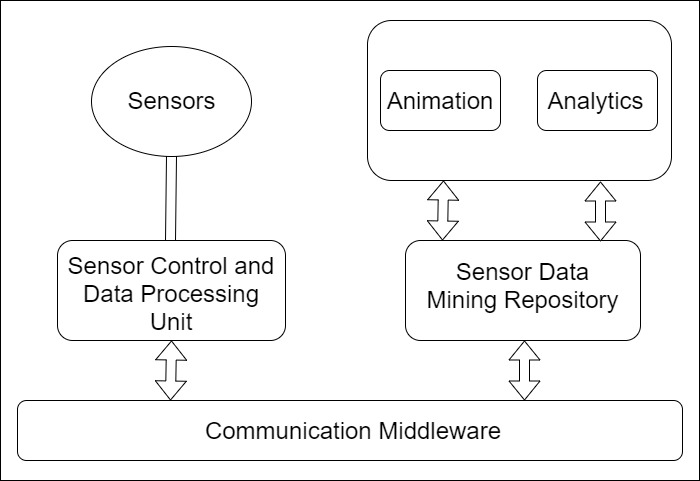
\includegraphics[scale=0.70]{images/figure2.png}
      \end{center}
      \caption{System Architecture}
      \label{overview}
  
    \end{figure}

    The hardware section includes multiple sensors, processor and also on the wireless communication module for transmitting and receiving signals. Second, we will discuss the air pollution software which mainly focuses on the visualization part. The overview of the system is as shown in the figure \ref{overview} and each part along with the sensor specification, implementation, design will be discussed further in the section. 


 \section{Hardware Architecture}
  
 \subsection{Sensor Control and Data Processing Unit}
This unit is the core for the pollution monitoring as it is where all the other modules are connected including the communication middleware. This module does the following function:


\begin{enumerate}

\item Control the sensors in collecting data.
\item It filters and processes the collected data and forward to the software.
\item Provide the necessary voltage for all the hardware connected to it.

\end{enumerate}
For simplicity and ease of programming we have selected one of the most popular processor in market, Arduino Ethernet board which has ATmega328 microcontroller as shown in Fig.\ref{Arduino}. 

\begin{figure}[h]
  \begin{center}
  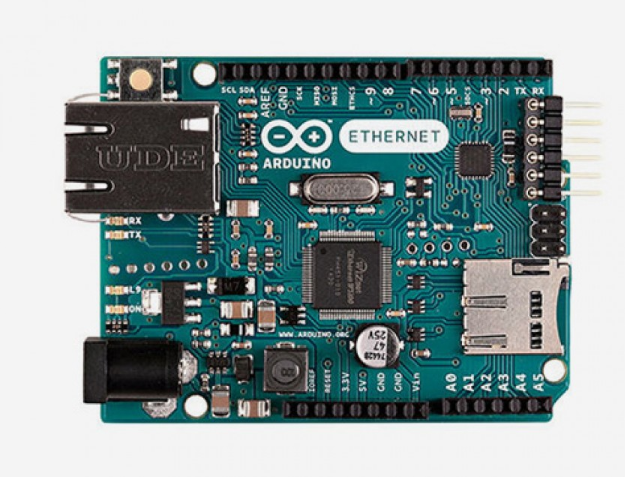
\includegraphics[scale=0.80]{./images/figure3.png}
  \end{center}
  \caption{Arduino Ethernet Board}
  \label{Arduino}
\end{figure}

Arduino is an open source physical computing platform that is divided into two parts, one is the hardware which is the board itself in which the external components are added to and other is the software which is the development environment for the  processing language. It is very easy and simple to use the board with any external devices such as sensors or actuators and is widely used by researchers. There are different features which makes arduino popular and can be listed as \cite{Banzi2008}:


\begin{enumerate}


  \item Arduino is multi-platform and can be used with windows,mac and linux.

  \item The programming is done via USB cable and not serial port and is useful as modern computers don't have serial port.

  \item As it is open source hardware and software all the necessity for an external hardware to be worked on like circuit diagram, the code can be easily downloaded.
  
  \item There is an Integrated Development Environment (IDE) which can be used as an interface for talking with the hardware and is very simple.
  
  \item There is an active arduino forum in which many researchers or developers who are working on projects contribute their ideas and will help in trouble shooting.
  
  \item The cost of the hardware is very cheap and will come under 60 CAD and is easily affordable.
  
\end{enumerate}

The board can be powered either by using a FTDI cable/USB serial connector, external power supply or using an optical Power Over ethernet module (PoE). The ATmega328 has 2 KB of SRAM and 1 KB of EEPROM. The detailed specification\cite{Guti2017} of the board is given below in the table \ref{table:Technical specification}.
 
\begin{table}[h]
  
  
  \begin{tabularx}{\columnwidth}{X|X}
      \hline
      Description                 & specification    \\
      \hline
      Microcontroller & ATmega328P \\
      Operating Voltage & 5V\\
      Input Voltage Plug (recommended) & 7-12V\\
      Input Voltage Plug (limits)       & 6-20V\\
      Input Voltage PoE (limits)        & 36-57V \\
      Digital I/O Pins    & 14 (of which 4 provide PWM output)     \\
      Analog Input Pins & 6\\
      Flash Memory & 32 KB (ATmega328P) of which 0.5 KB used by bootloader\\
      SRAM     & 2 KB (ATmega328P)\\
      EEPROM   & 1 KB (ATmega328P) \\
      Clock Speed  & 16 MHz\\
      \hline
    
  \end{tabularx}
  \caption{Technical specification}
  \label{table:Technical specification}
\end{table}
 

Having all these specification gives the freedom for researchers to explore with different electronic devices easily. The board is programmed with the help of arduino programming language which is very close to embedded C language and it is done on Arduino development environment. 

\subsection{Sensor}

Sensor networks are instruments useful to detect the conditions in remote places in the physical world in environmental monitoring applications such as pollution monitoring, transportation management, intrusion detection and many more \cite{Jung2011}. With constant development in electronics industry, it is possible to collect data remotely and collected data can be transferred to the required platform at a short period of time.
There are different sensors available in market which can measure the pollutants and display the value, but the idea here is to select the one which is of low cost and also gives the most accurate values.
\par
Having said that there is a variety of options available for sensors based on the way it measures the pollutants. One such category is Metal Oxide Semiconductor (MOS) gas sensor also known as semiconductor gas sensor, which is used to detect the concentration of any hazardous gases in the atmosphere by changing its resistance. The most popular series available in market for this category is MQ-XX sensors which is popular for its wide detecting scope, long life, stability, high sensitivity, fast response and also simple drive circuit \cite{Data2012}.The sensing material is made up either from Aluminum Oxide ($ Al_{2}O_{3}$) or Tungsten trioxide ($WO3$)based ceramic and has a coating of Tin Oxide $ SnO_{2} $ that acts as the sensing material for the desired gas. The sensing element is heated through Platinum wires which is connected to leads made up of Nickel-Chromium, well known conductive alloy. The gas to be detected has a specific temperature at which it gets ionized and the task of the sensor is to work at that temperature. Once the gas gets ionized it gets absorbed by the sensing material which changes the resistance and inturn changes the voltage across the sensor and can be read by the microcontroller \cite{gassensor}. The voltage value along with reference voltage and other resistor's resistance is used to find the resistance of sensor. Once the resistance of the sensor is known then by using the sensitivity curve the concentration could be found out. 

Another popularly used  MOS sensor which we explored was MICS which are MEMS based whose mode of operation is similar to the above said sensor as both of them are metal oxide. Here, oxidizing gas or the pollutant gas add to the insulative oxygen species causing the resistance to increase \cite{SGXSensortech}.
 Other than MOS sensors, we also took a look at optical sensor which are spectroscopic devices which uses light scattering principle to find the concentration of pollutants. These sensors are known for its detecting capability of particulate matter of different sizes and is one of the recent development in the field of air quality monitoring. Highly responsive, reliable and long life are the main highlights of this sensor.
 \subsubsection{Selected Sensor}

 After understanding the wide range of sensor options in the market the sensors were selected based on their performance, availability, ease of integration, and cost. The selected sensors were:
 \begin{enumerate}

  \item MQ-2 Sensor: This is a a semiconductor gas sensor which has an electrochemical sensor which detects multiple gases such as Carbon monoxide, LPG, methane, and other combustible steam. The sensor is connected in series with a variable resistor to form a voltage divider circuit and the variable resistor is used to change the sensitivity. The sensitivity curve for the sensor is shown for different types of gases.
\par
\begin{figure}[h]
  \begin{center}
  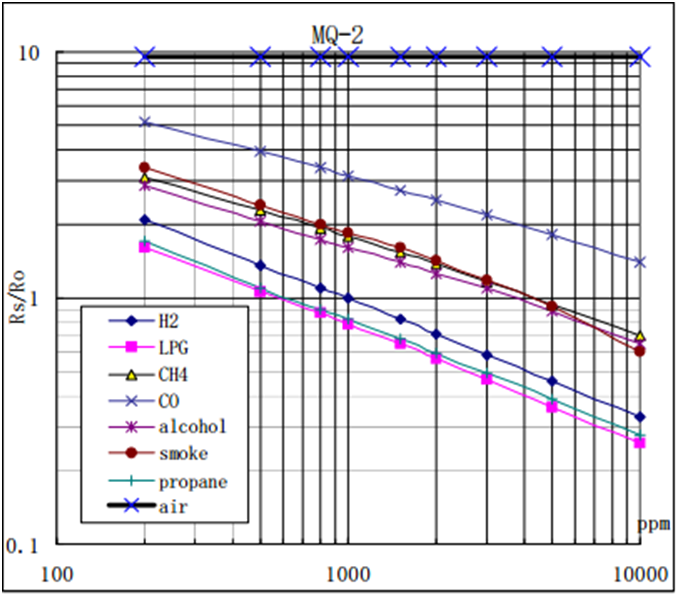
\includegraphics[scale=0.40]{./images/figure1.png}
  \end{center}
 
  \caption{Sensitivity characteristics curve \cite{Data2012}}
  
  \label{curve}
where $R_{o}$ is the sensor resistance in clean air and $R_{s}$ is the sensor resistance when exposed to gas.
\end{figure}
From the curve in Fig.\ref{curve}, the voltage across the sensor is found out depending on which gas one wants to detect and there after using this voltage value the concentration of pollutant is calculated. The range of detection of gas is from 100ppm to 10,000 ppm and has a high sensitivity and fast response time. The sensor is small and portable and provides integration in famous MCU platforms like arduino, raspberry pi etc. 

\item MQ 131: Another MQ-XX series sensor that we used for the system is for ozone. The working of the sensor is similar to MQ-2 sensor. It decreases the resistance when exposed to ozone and becomes more conductive when exposed to large concentration of the gas. This can be used to measure the concentration of ozone in air. The detecting concentration scope is from 10ppb to 2 ppm of ozone and also has a fast response time and long life.

\item MICS-2714: This is a robust MEMS sensor used for the detection of Nitrogen dioxide ($NO_2$). The detection range is from 0.05 to 10 ppm and has a response time of 10 seconds. The sensor is comparatively small and of low cost.

\item  PPD42NS Particulate sensor: The sensor detects the particulate matter through light scattering mechanism and consists of infrared LED positioned in forward angle to a photo diode. As soon as there is a variation in light density, the photo diode detects this and changes the current from the diode \cite{Allen2002}. The circuit generates a measurable signal known as Low Pulse Occupancy (LPO) which is proportional to PM concentration \cite{Kuula2017}. This sensor can measure both PM2.5 and PM10 concentration.

\item DHT11: This a very low cost sensor available in market for temperature and humidity measurement and has a calibrated digital output. The measurement range for temperature is from 0 degree to 50 degree Celsius. The device can be integrated to almost all platforms of Microcontroller and is considered to be the best choice for many applications.

 \end{enumerate}

 \subsection{Communication Middleware}
 
 The collected data needs to be transferred to the software so that user can understand and interpret the data from the sensor. Choosing the communication middleware was a tough task as we need a stable system that will constantly send data over the network. In the beginning we used an ESP module for this purpose. The WiFi module, ESP8266, which is a highly integrated SOC that meets the requirement of user demand of efficient power usage, compact design and reliable performance\cite{Systems2018}. The ESP module can be connected to a processor or it can also be flashed on its own as the module itself is a MCU unit. Unlike the other sensor modules connected to the processor which needs a 5V power supply for its working, this module needs a 3.3V for its power up. The ESP module comes along with installed firmware from AI-thinker and it can be communicated with AT commands. On typing the AT command in the serial monitor the output would come as 'OK' if there is a successful connection. 

 This firmware can be replaced with user's own code which gives the power of flexibility of connecting with any IOT platform. The arduino platform supports the programming of ESP module which makes the integration much easier. The code can be written in the Arduino IDE and can be flashed into the ESP board by connecting it separately.  However this module did not provide a reliable connection to the network and after few tests we had to replace it to another module. We choose a WEMOS[INSERT ABOUT WEMOS]
 
 \iffalse
 The circuit for the ESP flashing is as shown in figure \ref{cir} which is a voltage divider circuit.

 \begin{figure}[h]
  \begin{center}
  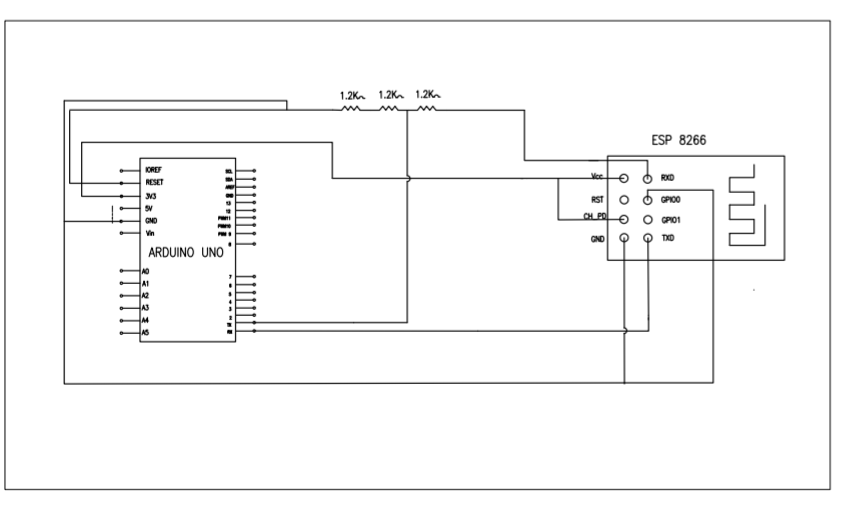
\includegraphics[scale=0.95]{./images/figure11.png}
  \end{center}
  \caption{System Overview}
  \label{cir}
\end{figure}


 When the TX and RX pin of arduino is connected to TX and RX pin of the WiFi module it becomes in the programming mode and flashing occurs. 
 \fi
 \subsection{System Overview}

 This section will show about the integration of the above mentioned sensors with the processor. After selecting the sensors and processor for the air pollution data measurement the next task was to put together so as to make it as a working system. This step was done one at a time so that troubleshooting will be easy. The complete circuit diagram of how the components are integrated to the Microcontroller is as shown is the figure\ref{circuit}.
 \begin{figure}[h]
  \begin{center}
  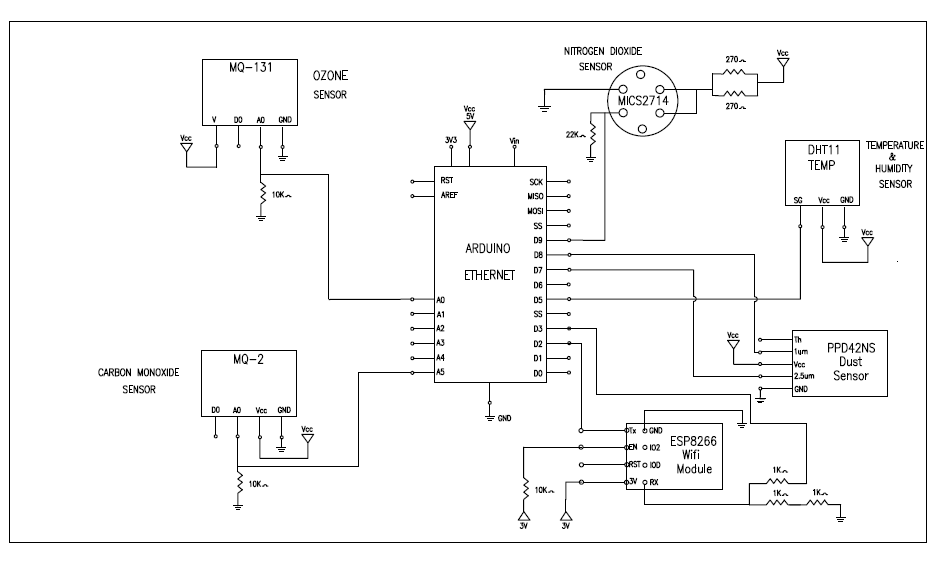
\includegraphics[scale=0.80]{./images/figure5.png}
  \end{center}
  \caption{Circuit daigram of air pollution system}
  \label{circuit}
\end{figure}
 Each of the sensors were carefully arranged so that it reduces the spatial interferences. As majority of the sensors are heat sensors and discharges heat it affects the working of the sensor placed near to each other. The figure \ref{prototype} shows the initial circuit implementation that was done in the breadboard with wires. Building the circuit in breadboard gave the flexibility of working with different arrangements.

 \begin{figure}[h]
  \begin{center}
  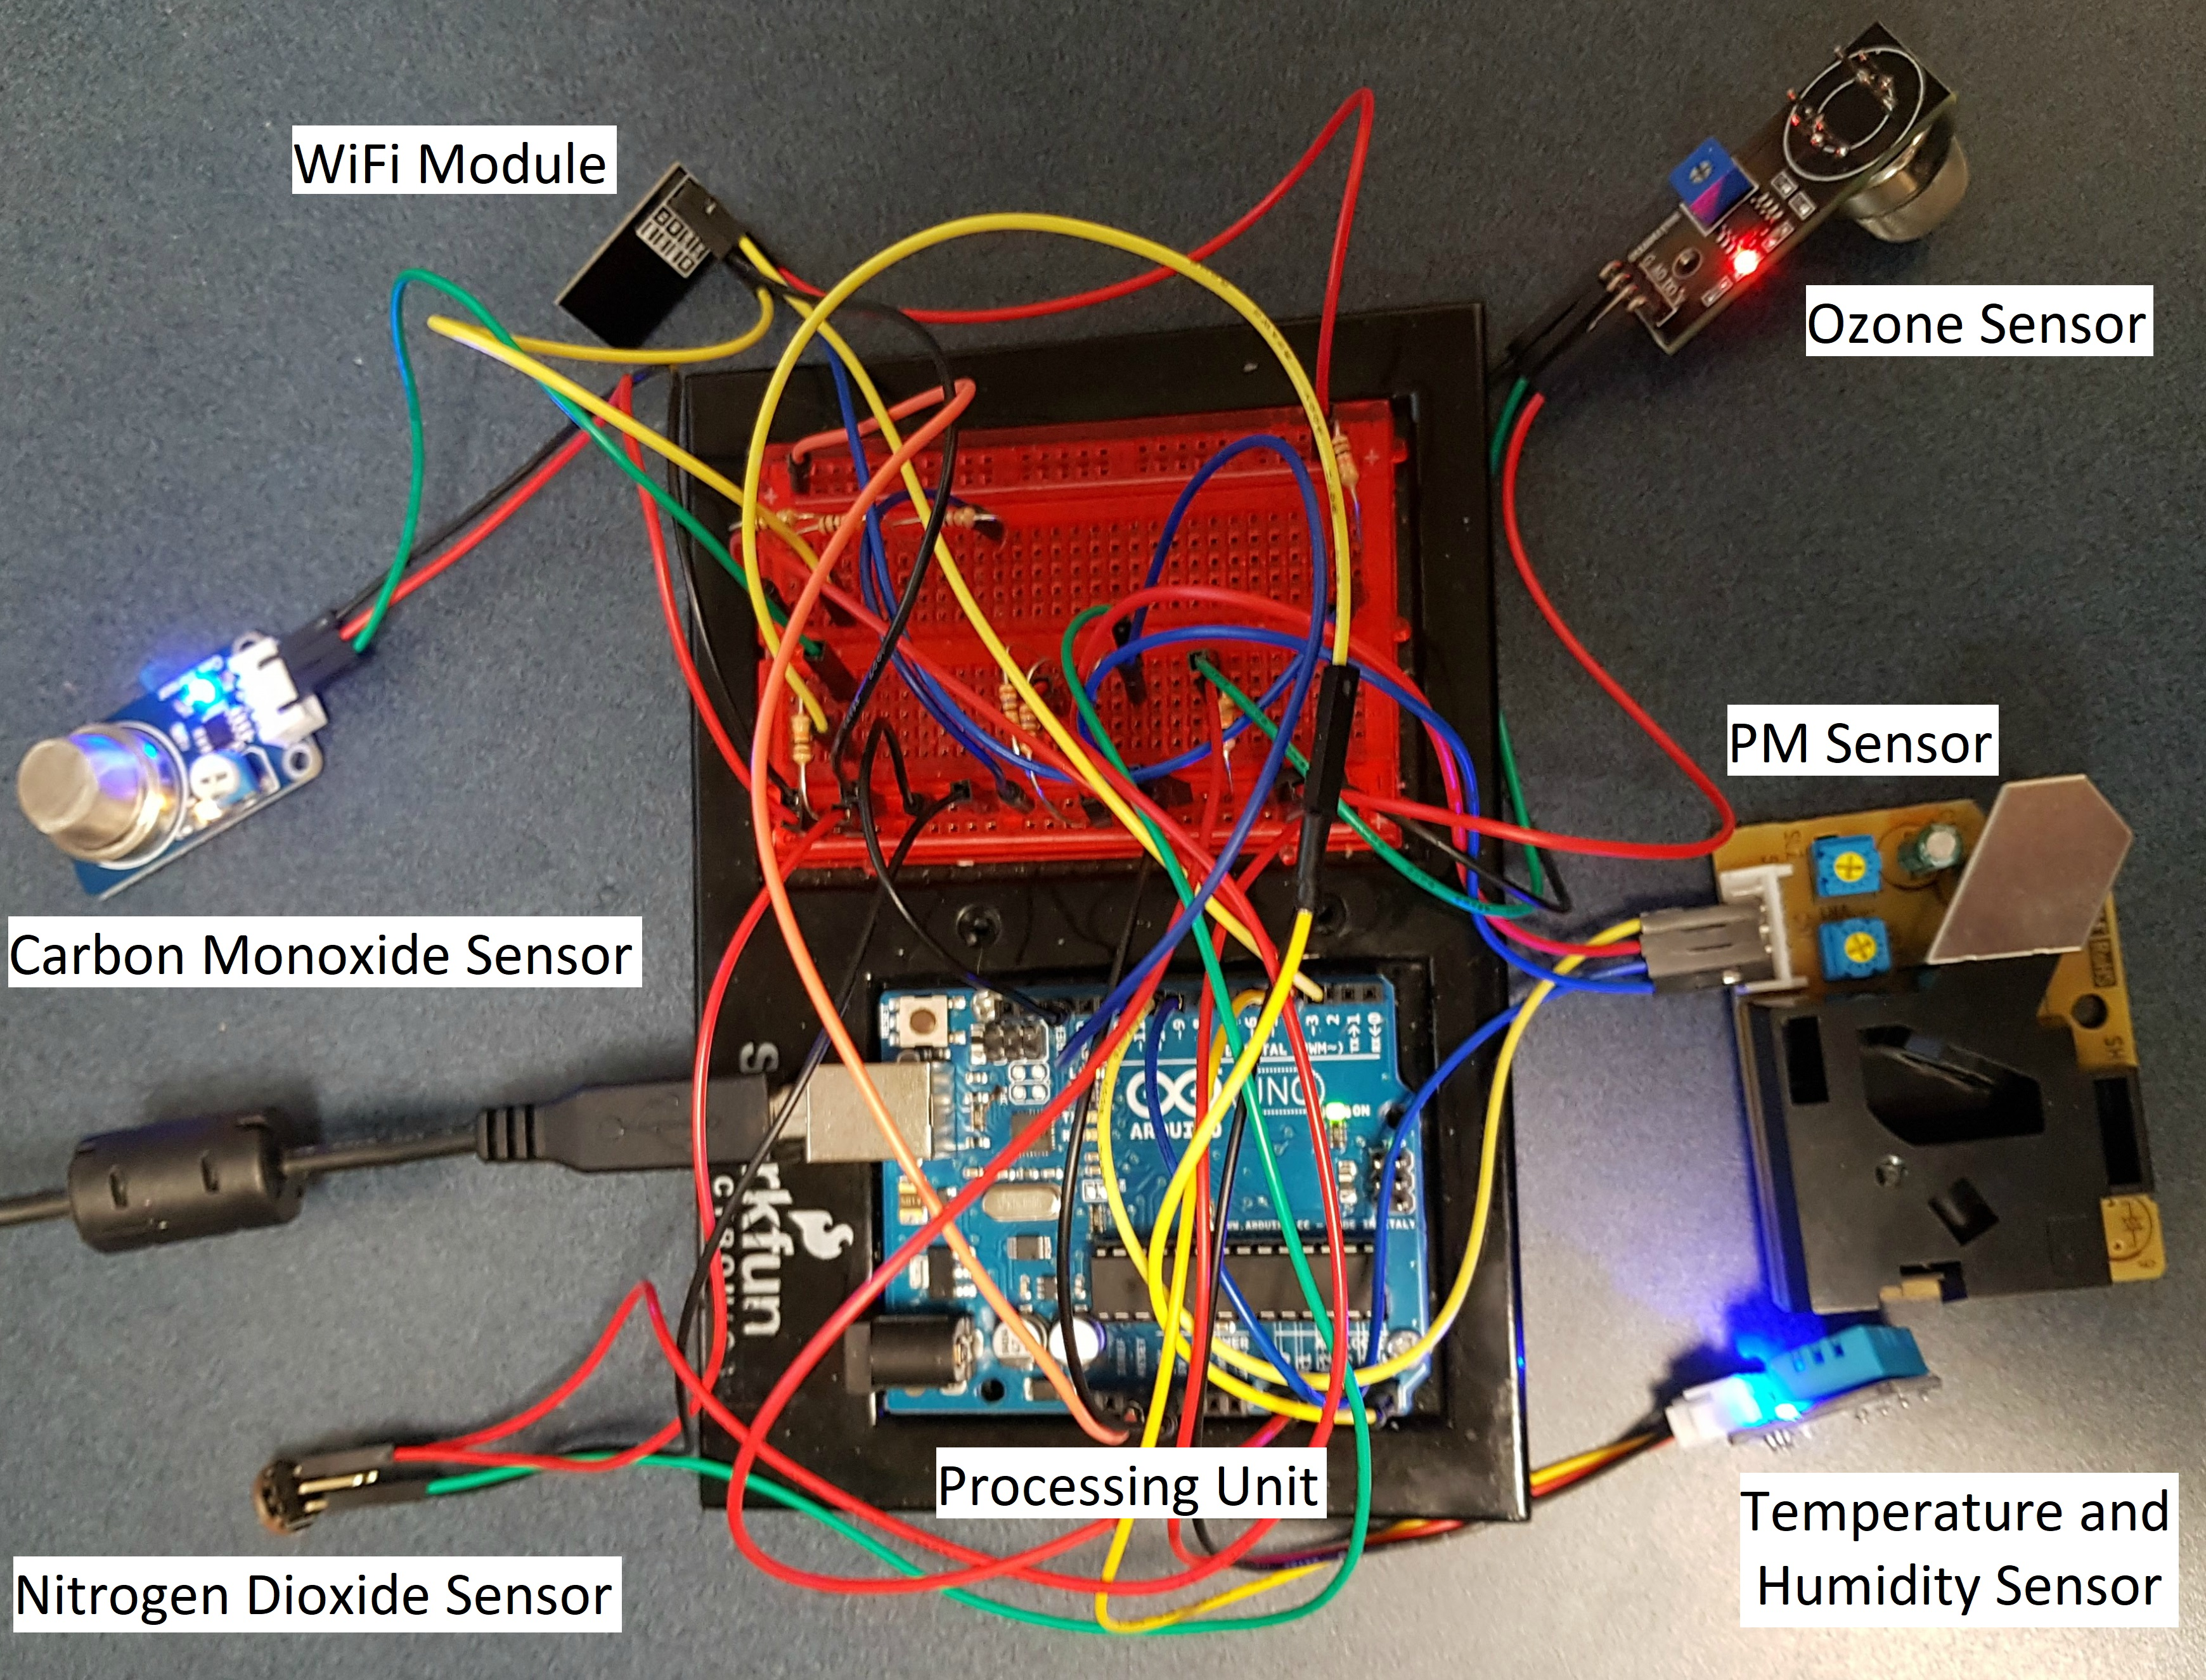
\includegraphics[scale=0.09]{./images/figure14.jpg}
  \end{center}
  \caption{Prototype Implementation}
  \label{prototype}
\end{figure}

After building the circuit in breadboard, it was migrated to a Printed Circuit Board (PCB) developed by Flemings Solution Ltd, India. The design of the board is as shown in the figure \ref{pcb}. The PCB was designed in such a way that each sensors and the microcontroller itself was plug-in model to board. 

\begin{figure}[h]
  \begin{center}
  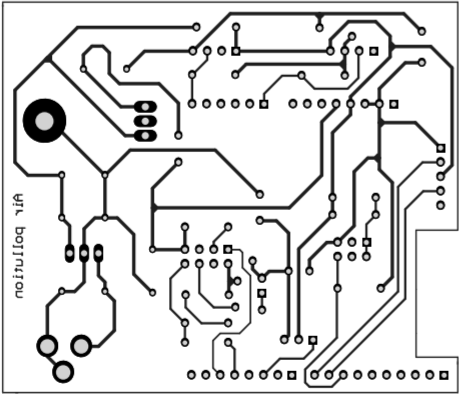
\includegraphics[scale=0.60]{./images/figure10.png}
  \end{center}
  \caption{Printed Circuit Board}
  \label{pcb}
\end{figure}

 This was done so that in case of any malfunctioning of any of the sensors or processor, it could be replaced easily. The main advantage of using a PCB design is that all the components are fixed and there is no wiring at all. This produces a zero error circuit and there wont be any short circuiting.

\section{Software Architecture : Customizable Layered Visualization (CLV)}

The hardware is the one responsible for the data collection but making these data available to user is done by an effective visualizing software. The main objective kept when developing the system was the data collected should be accessed from anywhere and thats why IoT platforms were selected. We developed a customizable layered visualization of data that potentially involve different stakeholders. We believe an effective visualization of concerned data is critically important for effectively combating major issues such as mentioned above. The software is driven by the following four key elements:

\begin{itemize}

\item Stakeholder specific  visualization.

\item Author-guided and user-driven interactiveness.

\item Hierarchical approach to visualization.

\item Providing alternate options.

\end{itemize}

\subsection{Framework}

"Seeing is believing because seeing is seduction"\cite{Hepworth}.

The pollution monitoring stations collect huge amount of data of pollutants and there are various ways to make people aware about these data. There can be different groups of users who will have access to these data which can be categorized as common people, educationist or the researchers who will be analyzing on the data, and the policy or law makers who will take necessary actions.

Accurately identifying all the stakeholders of air pollution is challenging. In \cite{English2000}, stakeholders in environmental risk decisions are identified into four categories of stakeholders as risk losers, risk gainers, risk perpetrators, risk managers. 
Risk losers in \cite{English2000} are those who may be adversely affected by environmental risk decision, in terms of health or economic values and risk gainers are those who may be favorably affected by an environmental risk decision, typically through economic gains. The people who create the risk are the perpetrators and those who takes the action against the risk are the risk managers. In a similar way, here we have put forward an approach of visualization based on the different stakeholders, in which we have classified into three categories: risk losers, risk analyzers and risk managers. 

Risk losers are those who are prone to pollution which include the common people or the society as a whole. Risk analyzers are those who identify the cause and increase in pollution and suggests pollution control methods. The next category is the one who implements laws and regulation by looking at the trends of pollution for a certain period of time, which are categorized as risk managers. 
We believe this categorization applies to air pollution too, and therefore based on this categorization we offer our data visualization strategy.

The visualization at first go should be very simple and be able to drive the user to which details they have to go through. It should not be representing all the data in a single screen which will be annoying to user and will end up loosing the interest of different stake holders. There should be options given to users so that the detailed data will be displayed. The user should be able to choose what data they need to view. If this approach is included in visualization, the data that different stakeholders are looking for will be passed onto them in a very efficient manner.

\subsection{Implementation of CLV of Air Pollution Data}

The complete software implementation of visualization was done with the combination of Node.js and python.The server used for storing the data from the system is Thingspeak \cite{thingspeak}. The collected data from the system is stored in the server of Thingspeak server \cite{thingspeak} which is a visualization paid service that was used for initial testing. 
According to the classification of stakeholders, each groups are looking for different kind of data. The data can be represented in the form of huge spreadsheets or documents. There are different methods for visualization like heat-maps, bubble plots, box plots, bar graphs or a plane graphs. The most common method of displaying the data is graphical method, which can show the data corresponding to a certain time or day. We believe that instead of visualizing the entire data through graphs or plots, it would be much easier for the public to interpret the data if it is a single instantaneous value. The  representation implemented for the first stakeholder which is the layman is as in figure \ref{view1}, which shows a single value of the pollutant which is all the data that as a citizen will be looking for.

\begin{figure}[h]
  \begin{center}
  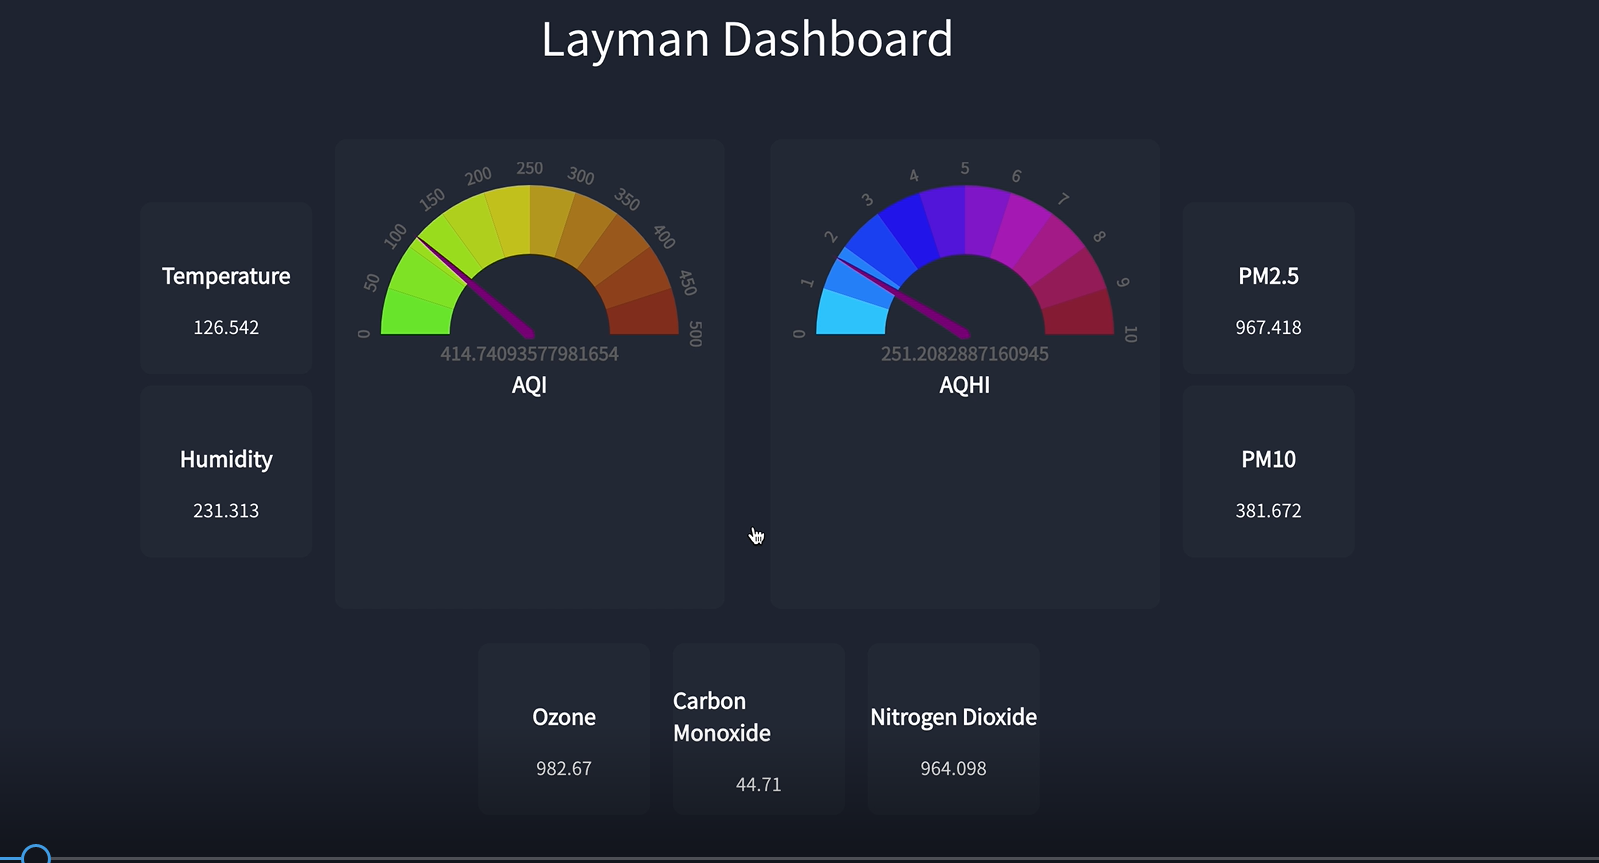
\includegraphics[scale=0.55]{./images/figure14.png}
  \end{center}
  \caption{Lay man view}
  \label{view1}
\end{figure}

The implemented representation is very easy to understand the data and it shows the concentration that each pollutant adds to atmosphere. The idea of this kind of visualization is that the user in the first category that is the common lay men, simply needs to read the data from display.
The next implentation is done for the  datascientist or researchers in figure \ref{view2} who need to get a detailed view of the collected data and time. The ideal way to represent detailed information is through a line graphs as it shows the value obtained for a given time. 

\begin{figure}[h]
  \begin{center}
  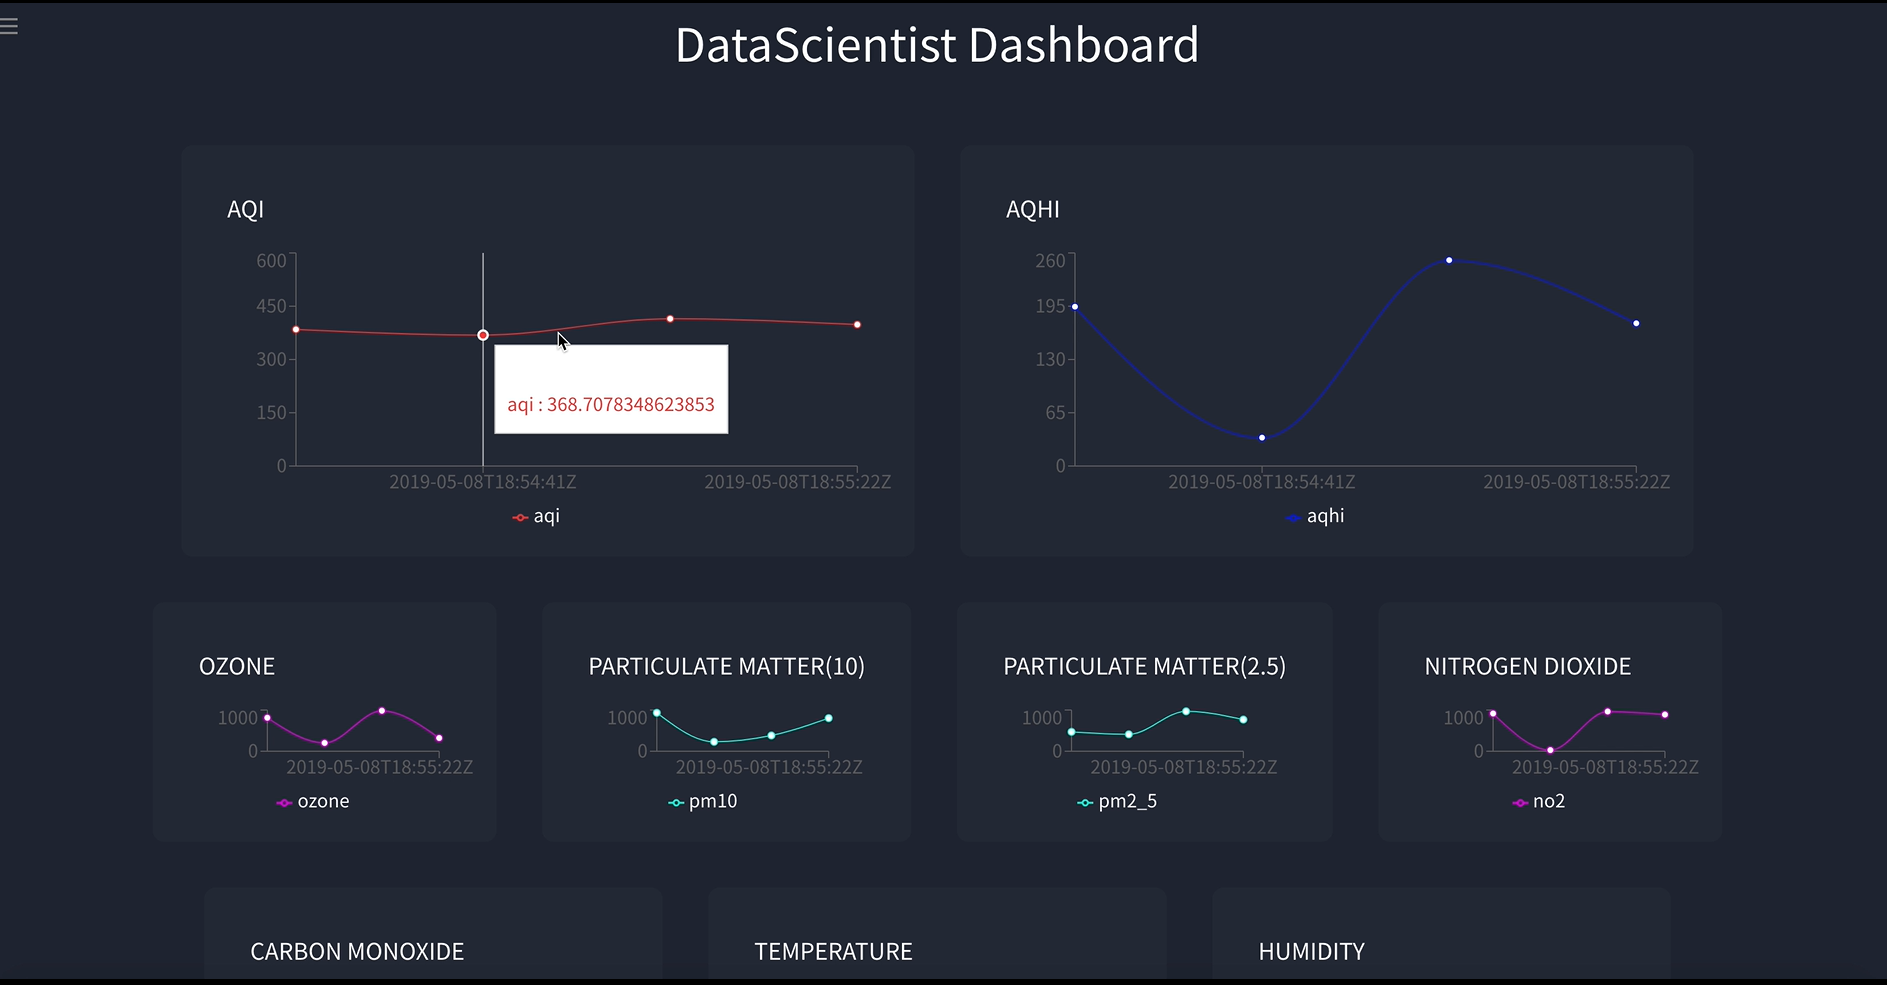
\includegraphics[scale=0.40]{./images/figure15.png}
  \end{center}
  \caption{Data Scientist view}
  \label{view2}
\end{figure}

The value of pollutant could be seen when the pointer is hovered over the graph. These graphs gets updated everytime when the data gets collected at the system as it is important for researchers to go through every collected data. The last categorization of the user is the policy makers who implements action against change in the concentration of pollutant. They are the once who enforce laws by looking at the pollutant data and hence they are the ones who need to see a combined view of all the pollutant as shown in figure \ref{view3} to understand the trend.

\begin{figure}[h]
  \begin{center}
  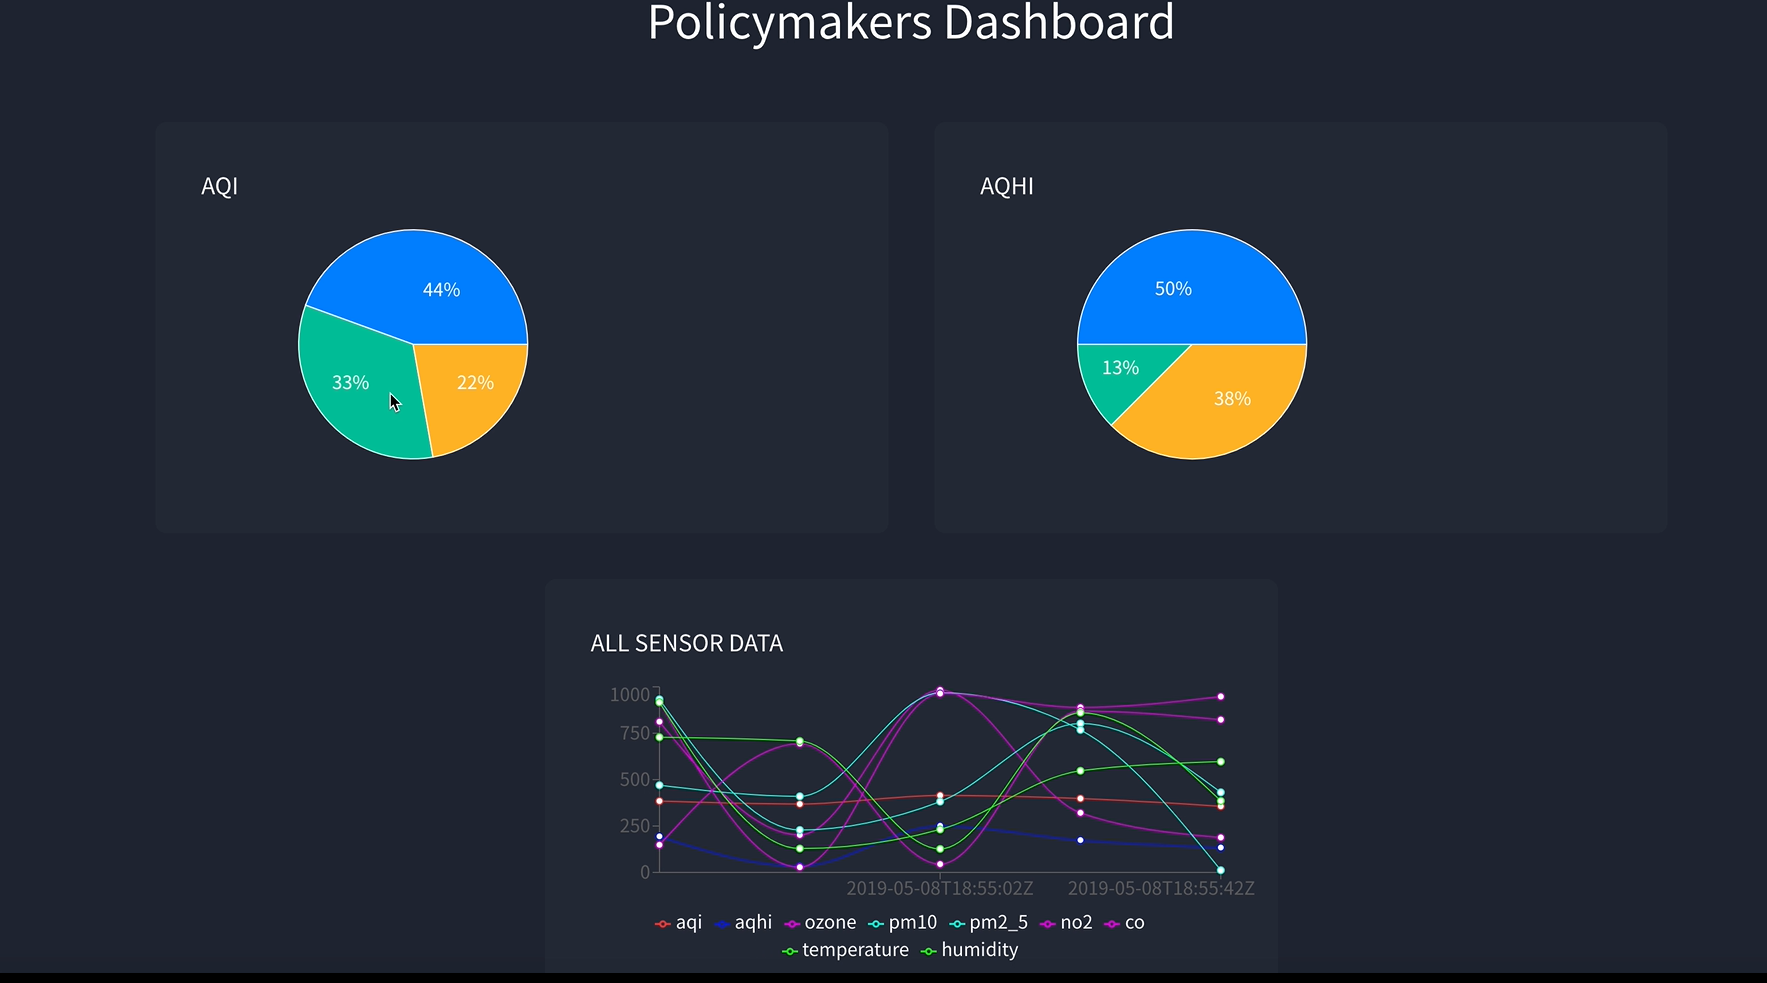
\includegraphics[scale=0.45]{./images/figure16.png}
  \end{center}
  \caption{Officials view}
  \label{view3}
\end{figure}

This can be viewed through a pie-chart which shows the percentage of each pollutant that contributes to the indexes.  There is also a combined line graph that shows the concentration of different pollutant data. By looking at the pie-charts and the combined graphs it would be easy to understand the trends and also could find the pollutant which contributes more to the developed indexes. 

The idea of such a hierarchial level of visualization is that it changes according to the people who are focusing on these data. Albert Cairo, a renowned information designer claims that the fundamental goal of data visualization should be to make people better informed \cite{Hepworth} \cite{Cairo2014},  similarly we also believe that a well communicated data is important for visualization.




\iffalse

We use an open source IoT platform called Thingspeak \cite{thingspeak}. It is integrated with the system to aggregate, analyze, visualize, and store the sensor
data that we collect \cite{thingspeak}. Thinkspeak can allow many users to integrate their system with other systems for collective and cooperative analysis of sensor data and promote citizen science in solving important global problems. It also offer a ‘hub’ model for data repository and a set of APIs for accessing and using the sensor data for their analysis and interpretations.
Thinkspeak provides an intuitive user interface that is easy to understand. It also provides a mobile application called Thingview which can be installed on our phone and the same data from the system can be visualized simultaneously.
For our purpose, we use Thinkspeak to display the results. As soon as the value is transferred to Thingspeak, it can immediately draw graph showing online visualization. We have used eight channels of Thingspeak for the graph representation of all the pollutants measured by the sensors and the AQI and AQHI metrics.

\fi